%!TEX root = /Users/louis/Documents/PhD/Deliverables/Thesis/thesis.tex

\section{Research Method}
\label{sec:research_method}
To explore the hypothesis outlined above, the thesis research was conducted using the method described in this section and summarised in Figure~\ref{fig:research_method}. The green boxes represent the three \emph{phases} of research, which are described below. The white boxes represent inputs and outputs to those phases.

%This section will discuss the way in which the research was conducted, including a description of the evaluation strategy.

% TODO - Need to highlight that lower level research objectives are identified in analysis and implementation chapters. This can probably also be explained in the method section 

\begin{figure}[htbp]
  \begin{center}
    \leavevmode
    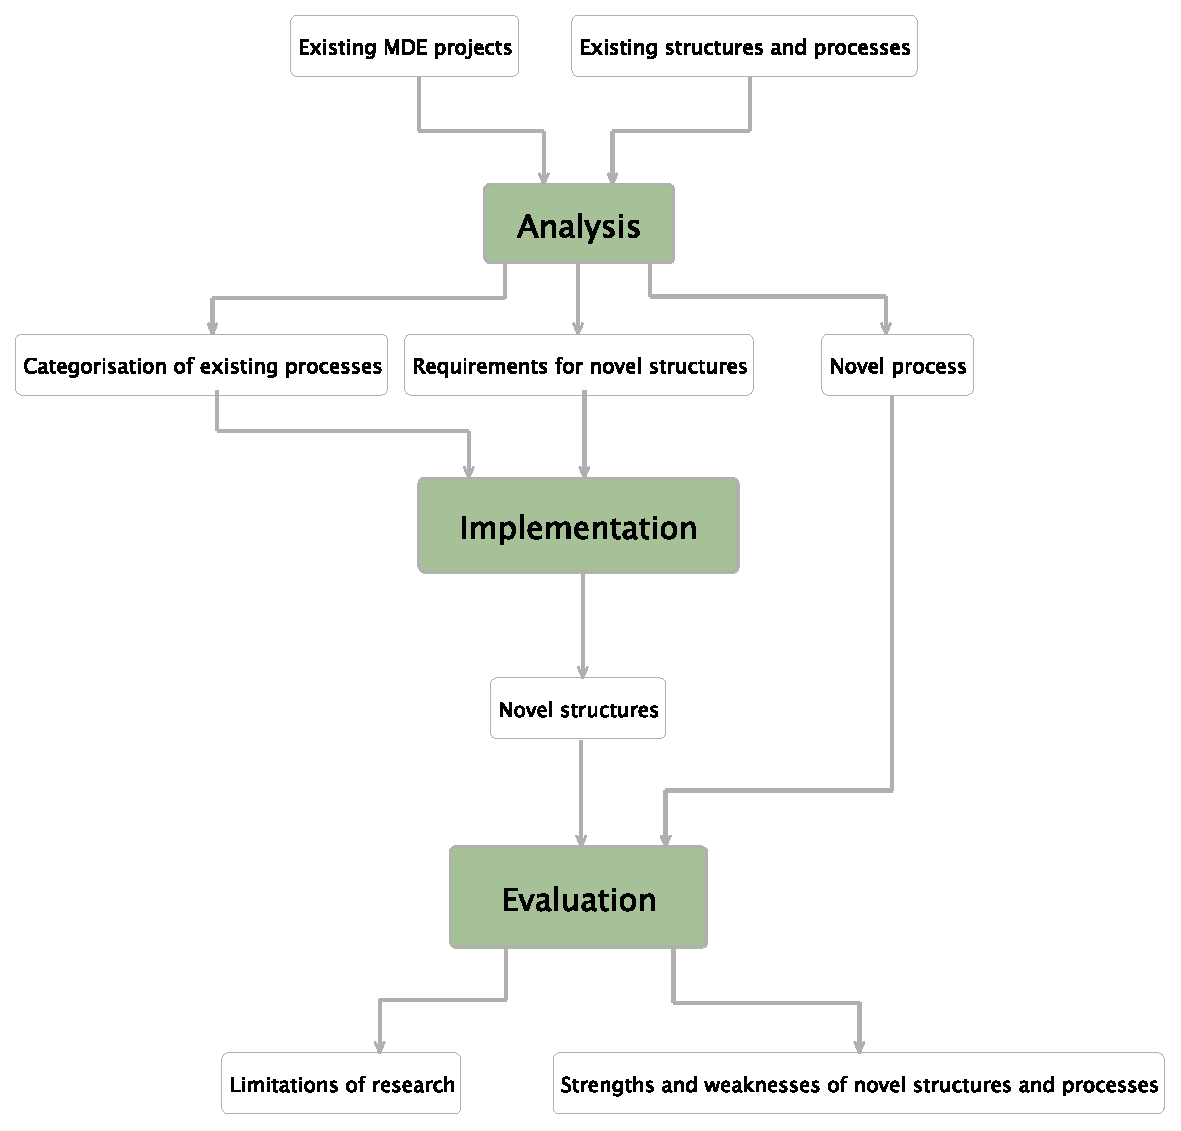
\includegraphics[width=12cm]{1.Introduction/images/method.pdf}
  \end{center}
  \caption{Overview of the research method.}
  \label{fig:research_method}
\end{figure}


Firstly, the \emph{analysis} phase involved identifying the ways in which evolution has occurred and has been identified and managed in existing MDE projects. The type of data obtained from the analysis phase determined the context in which the thesis research was conducted, model-metamodel co-evolution. Examples of evolution taken from existing MDE projects were used to investigate the strengths and weaknesses of existing structures and processes for identifying and managing evolution. Requirements for new structures and processes for identifying and managing evolution were formulated from the results of the analysis phase.

The \emph{implementation} phase involved designing and implementing novel structures and processes for identifying and managing evolution, and integrating the structures and processes with a contemporary MDE environment. The examples of evolution used in the analysis phase were used for testing the implementation of the structures and processes.

The \emph{evaluation} phase involved assessing the novel structures and processes for identifying and managing evolution by comparison to existing structures and processes. Evaluation was performed using examples of evolution from MDE projects. To mitigate a possible threat to the validity of the research, the examples used in the evaluation phase were different to those used in the analysis phase. The strengths and weaknesses of the novel and existing structures and processes were synthesised from the comparisons, particularly with respect to productivity, understandability and portability.

A similar method was used successfully in \cite{dig07thesis} to explore the extent to which component-based applications can be automatically evolved. Initially, \cite{dig06apis} conducted \emph{analysis} to identify and categorise evolution in five existing component-based applications, with the hypothesis that many of the changes could be classified as behaviour-preserving. By using examples from the survey, \cite{dig06detection} were able to \emph{implement} an algorithm for automatically detecting behaviour-preserving changes. The algorithm was then used to implement tools for (1) migrating code in a distributed and collaborative software development environment \cite{dig06automatic}, and (2) analysing the history of component-based applications \cite{dig07cms}. The latter facilitated better understanding of program evolution, and refinement of the detection algorithm. Finally, \cite{dig07thesis} \emph{evaluated} the tools and detection algorithm by application to three further component-based applications.